% Options for packages loaded elsewhere
\PassOptionsToPackage{unicode}{hyperref}
\PassOptionsToPackage{hyphens}{url}
%
\documentclass[
  man,floatsintext]{apa6}
\usepackage{amsmath,amssymb}
\usepackage{lmodern}
\usepackage{iftex}
\ifPDFTeX
  \usepackage[T1]{fontenc}
  \usepackage[utf8]{inputenc}
  \usepackage{textcomp} % provide euro and other symbols
\else % if luatex or xetex
  \usepackage{unicode-math}
  \defaultfontfeatures{Scale=MatchLowercase}
  \defaultfontfeatures[\rmfamily]{Ligatures=TeX,Scale=1}
\fi
% Use upquote if available, for straight quotes in verbatim environments
\IfFileExists{upquote.sty}{\usepackage{upquote}}{}
\IfFileExists{microtype.sty}{% use microtype if available
  \usepackage[]{microtype}
  \UseMicrotypeSet[protrusion]{basicmath} % disable protrusion for tt fonts
}{}
\makeatletter
\@ifundefined{KOMAClassName}{% if non-KOMA class
  \IfFileExists{parskip.sty}{%
    \usepackage{parskip}
  }{% else
    \setlength{\parindent}{0pt}
    \setlength{\parskip}{6pt plus 2pt minus 1pt}}
}{% if KOMA class
  \KOMAoptions{parskip=half}}
\makeatother
\usepackage{xcolor}
\usepackage{graphicx}
\makeatletter
\def\maxwidth{\ifdim\Gin@nat@width>\linewidth\linewidth\else\Gin@nat@width\fi}
\def\maxheight{\ifdim\Gin@nat@height>\textheight\textheight\else\Gin@nat@height\fi}
\makeatother
% Scale images if necessary, so that they will not overflow the page
% margins by default, and it is still possible to overwrite the defaults
% using explicit options in \includegraphics[width, height, ...]{}
\setkeys{Gin}{width=\maxwidth,height=\maxheight,keepaspectratio}
% Set default figure placement to htbp
\makeatletter
\def\fps@figure{htbp}
\makeatother
\setlength{\emergencystretch}{3em} % prevent overfull lines
\providecommand{\tightlist}{%
  \setlength{\itemsep}{0pt}\setlength{\parskip}{0pt}}
\setcounter{secnumdepth}{-\maxdimen} % remove section numbering
% Make \paragraph and \subparagraph free-standing
\ifx\paragraph\undefined\else
  \let\oldparagraph\paragraph
  \renewcommand{\paragraph}[1]{\oldparagraph{#1}\mbox{}}
\fi
\ifx\subparagraph\undefined\else
  \let\oldsubparagraph\subparagraph
  \renewcommand{\subparagraph}[1]{\oldsubparagraph{#1}\mbox{}}
\fi
\newlength{\cslhangindent}
\setlength{\cslhangindent}{1.5em}
\newlength{\csllabelwidth}
\setlength{\csllabelwidth}{3em}
\newlength{\cslentryspacingunit} % times entry-spacing
\setlength{\cslentryspacingunit}{\parskip}
\newenvironment{CSLReferences}[2] % #1 hanging-ident, #2 entry spacing
 {% don't indent paragraphs
  \setlength{\parindent}{0pt}
  % turn on hanging indent if param 1 is 1
  \ifodd #1
  \let\oldpar\par
  \def\par{\hangindent=\cslhangindent\oldpar}
  \fi
  % set entry spacing
  \setlength{\parskip}{#2\cslentryspacingunit}
 }%
 {}
\usepackage{calc}
\newcommand{\CSLBlock}[1]{#1\hfill\break}
\newcommand{\CSLLeftMargin}[1]{\parbox[t]{\csllabelwidth}{#1}}
\newcommand{\CSLRightInline}[1]{\parbox[t]{\linewidth - \csllabelwidth}{#1}\break}
\newcommand{\CSLIndent}[1]{\hspace{\cslhangindent}#1}
\ifLuaTeX
\usepackage[bidi=basic]{babel}
\else
\usepackage[bidi=default]{babel}
\fi
\babelprovide[main,import]{english}
% get rid of language-specific shorthands (see #6817):
\let\LanguageShortHands\languageshorthands
\def\languageshorthands#1{}
% Manuscript styling
\usepackage{upgreek}
\captionsetup{font=singlespacing,justification=justified}

% Table formatting
\usepackage{longtable}
\usepackage{lscape}
% \usepackage[counterclockwise]{rotating}   % Landscape page setup for large tables
\usepackage{multirow}		% Table styling
\usepackage{tabularx}		% Control Column width
\usepackage[flushleft]{threeparttable}	% Allows for three part tables with a specified notes section
\usepackage{threeparttablex}            % Lets threeparttable work with longtable

% Create new environments so endfloat can handle them
% \newenvironment{ltable}
%   {\begin{landscape}\centering\begin{threeparttable}}
%   {\end{threeparttable}\end{landscape}}
\newenvironment{lltable}{\begin{landscape}\centering\begin{ThreePartTable}}{\end{ThreePartTable}\end{landscape}}

% Enables adjusting longtable caption width to table width
% Solution found at http://golatex.de/longtable-mit-caption-so-breit-wie-die-tabelle-t15767.html
\makeatletter
\newcommand\LastLTentrywidth{1em}
\newlength\longtablewidth
\setlength{\longtablewidth}{1in}
\newcommand{\getlongtablewidth}{\begingroup \ifcsname LT@\roman{LT@tables}\endcsname \global\longtablewidth=0pt \renewcommand{\LT@entry}[2]{\global\advance\longtablewidth by ##2\relax\gdef\LastLTentrywidth{##2}}\@nameuse{LT@\roman{LT@tables}} \fi \endgroup}

% \setlength{\parindent}{0.5in}
% \setlength{\parskip}{0pt plus 0pt minus 0pt}

% Overwrite redefinition of paragraph and subparagraph by the default LaTeX template
% See https://github.com/crsh/papaja/issues/292
\makeatletter
\renewcommand{\paragraph}{\@startsection{paragraph}{4}{\parindent}%
  {0\baselineskip \@plus 0.2ex \@minus 0.2ex}%
  {-1em}%
  {\normalfont\normalsize\bfseries\itshape\typesectitle}}

\renewcommand{\subparagraph}[1]{\@startsection{subparagraph}{5}{1em}%
  {0\baselineskip \@plus 0.2ex \@minus 0.2ex}%
  {-\z@\relax}%
  {\normalfont\normalsize\itshape\hspace{\parindent}{#1}\textit{\addperi}}{\relax}}
\makeatother

% \usepackage{etoolbox}
\makeatletter
\patchcmd{\HyOrg@maketitle}
  {\section{\normalfont\normalsize\abstractname}}
  {\section*{\normalfont\normalsize\abstractname}}
  {}{\typeout{Failed to patch abstract.}}
\patchcmd{\HyOrg@maketitle}
  {\section{\protect\normalfont{\@title}}}
  {\section*{\protect\normalfont{\@title}}}
  {}{\typeout{Failed to patch title.}}
\makeatother

\usepackage{xpatch}
\makeatletter
\xapptocmd\appendix
  {\xapptocmd\section
    {\addcontentsline{toc}{section}{\appendixname\ifoneappendix\else~\theappendix\fi\\: #1}}
    {}{\InnerPatchFailed}%
  }
{}{\PatchFailed}
\keywords{attractiveness, simulation monitoring, fiction, deep fakes, sense of reality\newline\indent Word count: 4088}
\usepackage{lineno}

\linenumbers
\usepackage{csquotes}
\usepackage[titles]{tocloft}
\cftpagenumbersoff{figure}
\renewcommand{\cftfigpresnum}{\itshape\figurename\enspace}
\renewcommand{\cftfigaftersnum}{.\space}
\setlength{\cftfigindent}{0pt}
\setlength{\cftafterloftitleskip}{0pt}
\settowidth{\cftfignumwidth}{Figure 10.\qquad}
\usepackage[labelfont=bf, font={scriptsize, color=gray}]{caption}
\ifLuaTeX
  \usepackage{selnolig}  % disable illegal ligatures
\fi
\IfFileExists{bookmark.sty}{\usepackage{bookmark}}{\usepackage{hyperref}}
\IfFileExists{xurl.sty}{\usepackage{xurl}}{} % add URL line breaks if available
\urlstyle{same} % disable monospaced font for URLs
\hypersetup{
  pdftitle={Too Beautiful to be Fake: Attractive Faces are Less Likely to be Judged as Artificially Generated},
  pdfauthor={Dominique Makowski1, An Shu Te1, Stephanie Kirk1, Ngoi Zi Liang1, Panagiotis Mavros2, \& S.H. Annabel Chen1, 3, 4, 5},
  pdflang={en-EN},
  pdfkeywords={attractiveness, simulation monitoring, fiction, deep fakes, sense of reality},
  hidelinks,
  pdfcreator={LaTeX via pandoc}}

\title{\textbf{Too Beautiful to be Fake: Attractive Faces are Less Likely to be Judged as Artificially Generated}}
\author{Dominique Makowski\textsuperscript{1}, An Shu Te\textsuperscript{1}, Stephanie Kirk\textsuperscript{1}, Ngoi Zi Liang\textsuperscript{1}, Panagiotis Mavros\textsuperscript{2}, \& S.H. Annabel Chen\textsuperscript{1, 3, 4, 5}}
\date{}


\shorttitle{Attractiveness and Reality}

\authornote{

Correspondence concerning this article should be addressed to Dominique Makowski, HSS 04-18, 48 Nanyang Avenue, Singapore (\href{mailto:dom.makowski@gmail.com}{\nolinkurl{dom.makowski@gmail.com}}).

The authors made the following contributions. Dominique Makowski: Conceptualization, Data curation, Formal Analysis, Funding acquisition, Investigation, Methodology, Project administration, Resources, Software, Supervision, Validation, Visualization, Writing -- original draft; An Shu Te: Data curation, Project administration, Resources, Investigation, Writing -- original draft; Stephanie Kirk: Project administration, Resources, Writing -- original draft; Ngoi Zi Liang: Project administration, Resources, Writing -- review \& editing; Panagiotis Mavros: Supervision, Writing -- review \& editing; S.H. Annabel Chen: Project administration, Supervision, Writing -- review \& editing.

Correspondence concerning this article should be addressed to Dominique Makowski, HSS 04-18, 48 Nanyang Avenue, Singapore. E-mail: \href{mailto:dom.makowski@gmail.com}{\nolinkurl{dom.makowski@gmail.com}}

}

\affiliation{\vspace{0.5cm}\textsuperscript{1} School of Social Sciences, Nanyang Technological University, Singapore\\\textsuperscript{2} Singapore-ETH Centre, Future Cities Laboratory, Singapore\\\textsuperscript{3} LKC Medicine, Nanyang Technological University, Singapore\\\textsuperscript{4} National Institute of Education, Singapore\\\textsuperscript{5} Centre for Research and Development in Learning, Nanyang Technological University, Singapore}

\abstract{%
Technological advances render the distinction between artificial (e.g., computer-generated faces) and real stimuli increasingly difficult, yet the factors driving our beliefs regarding the nature of ambiguous stimuli remain largely unknown. In this study, 150 participants rated 109 pictures of faces on 4 characteristics (attractiveness, beauty, trustworthiness, familiarity). The stimuli were then presented again with the new information that some of them were AI-generated, and participants had to rate each image according to whether they believed them to be real or fake. Strikingly, despite all images being pictures of real faces from the same database, most participants rated a large portion of them as ``fake''. Moreover, our results suggest a gender-dependent role of attractiveness on reality judgements, with faces rated as more attractive being classified as more real. We also report links between reality beliefs tendencies and dispositional traits such as narcissism and paranoid ideation.
}



\begin{document}
\maketitle

For the first time in human history, technology has enabled the creation of near-perfect simulations indistinguishable from reality. These artificial, yet realistic constructs permeate all areas of life through immersive works of fiction, deep fakes (real-like images and videos generated by deep learning algorithms), virtual and augmented reality (VR and AR), artificial beings (artificial intelligence ``bots'' with or without a physical form), fake news and skewed narratives, of which ground truth is often hard to access (Nightingale \& Farid, 2022). Such developments not only carry important consequences for the technological and entertainment sectors, but also for security and politics - for instance if used for propaganda and disinformation, recruitment into malevolent organizations, or religious indoctrination (Pantserev, 2020). This issue is central to what has been coined the ``post-truth era'' (Lewandowsky et al., 2017), in which the distinction (and lack thereof) between authentic and simulated objects will play a critical role.

While not all simulations have achieved perfect realism (e.g., Computer Generated Images - CGI in movies often lack certain key details that makes them visually distinct from real images, McDonnell \& Breidt, 2010), it is fair to assume that these technical limitations will become negligible in the near future, particularly in the field of face generation (Moshel et al., 2022; Nightingale \& Farid, 2022; Tucciarelli et al., 2020). Such performance, however, leads to a new question: if real and fake stimuli cannot be distinguished based on their objective characteristics, how can we make judgements regarding their nature?

Literature shows that the context surrounding a stimulus often plays an important role in the assessment of its reality (a process henceforth referred to as \emph{simulation monitoring}, Makowski, 2018; Makowski, Sperduti, et al., 2019). With the extensive search and processing of cues within ambiguous stimuli being an increasingly complex and cognitively effortful strategy (Michael \& Sanson, 2021; Susmann et al., 2021), people tend to draw on peripheral contextual cues (\textbf{Figure 1}), such as the source of the stimulus (e.g., in what journal has information been published), and its credibility, authority and expertise, to help facilitate their evaluation (Michael \& Sanson, 2021; Petty \& Cacioppo, 1986; Susmann et al., 2021). However, the automization and decontextualization of information allowed by online social media (where text snippets or video excerpts are mass-shared with little context) makes this task increasingly difficult (Berghel, 2018; Y. Chen et al., 2015). Thus, in the absence of clear contextual information, what drives our beliefs of reality?

\begin{figure}
\includegraphics[width=1\linewidth]{../figures/Figure1} \caption{The decision to believe that an ambiguous stimulus (of any form, e.g., images, text, videos, environments, ...) is real or fake depends of individual characteristics (e.g., personality and cognitive styles), stimulus-related features (context, emotionality), and their interaction, which can manifest for instance in our bodily reaction.}\label{fig:unnamed-chunk-2}
\end{figure}

Evidence suggests that inter-individual characteristics play a crucial role in simulation monitoring, with factors such as cognitive style, prior beliefs, and personality traits (Bryanov \& Vziatysheva, 2021; Ecker et al., 2022; Sindermann et al., 2020). For instance, individuals with stronger analytical reasoning have been found to better discriminate real from fake stimuli (Pehlivanoglu et al., 2021; Pennycook \& Rand, 2019), and prior knowledge or beliefs about the stimulus influences one's perception of it by biasing the attention deployment towards information that is in line with one's expectations (Britt et al., 2019). Furthermore, dispositional traits, such as high levels of narcissism and low levels of openness and conscientiousness, have been associated with greater susceptibility to fake news (Piksa et al., 2022; Sindermann et al., 2020).

Beyond stimulus- and individual-related characteristics, evidence suggests that the interaction between the two (i.e., the subjective reaction associated with the experience of a given stimulus), contributes to simulation monitoring decisions. For instance, the intensity of experienced emotions have been shown to increase one's sense of presence - the extent to which one feels like ``being there'', as if the object of experience was real - when engaged in a fictional movie or a VR environment (Makowski et al., 2017; Sanchez-Vives \& Slater, 2005). Conversely, beliefs that emotional stimuli were fake (e.g., that emotional scenes were not authentic but instead involved actors and movie makeup) were found to result in emotion down-regulation (Makowski, Sperduti, et al., 2019; Sperduti et al., 2017). In line with these findings, studies on susceptibility to fake news have also found heightened stimulus emotionality to be associated with greater belief (Bago et al., 2022; Martel et al., 2020). Additionally, other factors, such as the stimuli's perceived self-relevance (Goldstein, 2009; Sperduti et al., 2016), as well as familiarity (Begg et al., 1992), could also play a role in guiding our appraisal of a stimulus.

AI-generated images of faces, due to their popularity as a target of CGI technology and to the possibility of experimentally manipulating facial features, are increasingly used to study face processing in relationship with saliency or emotions, as well as to other important components of face evaluation, such as trustworthiness or attractiveness (Balas \& Pacella, 2017; Calbi et al., 2017; Sobieraj \& Krämer, 2014; Tsikandilakis et al., 2019). Interestingly, artificially created faces rated as more attractive (by an independent group of raters) were perceived as less real (Tucciarelli et al., 2020). Conversely, Liefooghe et al. (2022) reports that attractiveness ratings were significantly lower when participants who were told that the faces were AI-generated were compared to those who had no prior knowledge. Whereas this line of evidence suggests that reality beliefs have an effect on face attractiveness ratings, the opposite question - whether attractiveness could drive simulation monitoring - has received little attention to date.

This study primarily aims at exploring the effect of facial attractiveness on simulation monitoring, i.e., on the beliefs that an image is real or artificially generated. Based on the embodied reality theory
(outlined in Makowski, 2018; Makowski, Sperduti, et al., 2019),
which suggests that salient and emotional stimuli are perceived to be more real, we hypothesize a quadratic relationship between perceived realness and attractiveness: faces rated as highly attractive or unattractive will more likely be believed to be real. We expect a similar relationship with trustworthiness ratings given its well-established link with attractiveness (Bartosik et al., 2021; Garrido \& Prada, 2017; Liefooghe et al., 2022; Little et al., 2011), and a positive relationship with familiarity (as more familiar faces would appear as more salient, self-relevant and anchored in reality). Additionally, we will further explore the link shared by dispositional traits, such as personality and attitude towards AI, with simulation monitoring tendencies. This study aims beyond the investigation of the discriminative accuracy between ``true'' photos and ``true'' artificially-generated images, focusing on the beliefs that a stimulus is real or fake, independently of its true nature.

\hypertarget{methods}{%
\subsection{Methods}\label{methods}}

\hypertarget{ethics-statement}{%
\subsubsection{Ethics Statement}\label{ethics-statement}}

This study was approved by the NTU Institutional Review Board (NTU IRB-2022-187) and all procedures performed were in accordance with the ethical standards of the institutional board and with the 1964 Helsinki Declaration. All participants provided their informed consent prior to participation and were incentivized after completing the study.

\hypertarget{procedure}{%
\subsubsection{Procedure}\label{procedure}}

In the first part of the study, participants answered a series of personality questionnaires, including the \emph{Mini-IPIP6}
(24 items, Sibley et al., 2011)
measuring 6 personality traits, the \emph{SIAS-6} and the \emph{SPS-6}
(6 items each, Peters et al., 2012)
assessing social anxiety levels, the \emph{FFNI-BF}
(30 items, Jauk et al., 2022)
measuring 9 facets of narcissism; the \emph{R-GPTS}
(18 items, Freeman et al., 2021)
measuring 2 dimensions related to paranoid thinking; and the \emph{IUS-12}
(12 items, Carleton et al., 2007)
measuring intolerance to uncertainty. Self-rated attractiveness was also assessed using 2 items - one measuring general attractiveness
(``How attractive would you say you are?'' Marcinkowska et al., 2021)
and the other measuring physical attractiveness
(``How would you rate your own physical attractiveness relative to the average,'' Spielmann et al., 2020).
Finally, we devised 5 items pertaining to expectations about AI-generated image technology (``I think current Artificial Intelligence algorithms can generate very realistic images''). To lower their saliency and the possibility of it priming the subjects about the task, we mixed these items with 5 items from the general attitudes towards AI scale
(\emph{GAAIS}, Schepman \& Rodway, 2020).
This scale was presented after the social anxiety questionnaires. 3 attention check questions were also embedded in the surveys.

In the second part of this study, 109 images of neutral-expression faces from the validated American Multiracial Face Database
(AMFD, J. M. Chen et al., 2021)
were presented to the participants for 500ms each, in a randomized order, following a fixation cross display (750 ms). After each stimulus presentation, ratings of \emph{Trustworthiness} (``I find this person trustworthy'') and \emph{Familiarity} (``This person reminds me of someone I know'') were collected using visual analog scales. Notably, as facial attractiveness is a multidimensional construct, encompassing evolutionary, sociocultural, biological as well as cognitive aspects (Han et al., 2018; Rhodes et al., 2006), we assessed attractiveness using 2 visual analog scales, measuring general \emph{Attractiveness} (``I find this person attractive'') and physical \emph{Beauty} (``This face is good-looking'').

In the last part of the study, participants were informed that ``about half'' of the images previously seen were AI-generated (the instructions used a cover story explaining that the aim of the research was to validate a new face generation algorithm). The same set of stimuli was displayed again for 500 ms in a new randomized order. This time, after each display, participants were asked to express their belief regarding the nature of the stimulus using a visual analog scale (with \emph{Fake} and \emph{Real} as the two extremes). The study was implemented using \emph{jsPsych} (De Leeuw, 2015), and the exact instructions are available in the experiment code.

\hypertarget{participants}{%
\subsubsection{Participants}\label{participants}}

One hundred and fifty participants were recruited via \emph{Prolific}, a crowd-sourcing platform recognized for providing high quality data (Peer et al., 2022). The only inclusion criterion was a fluent proficiency in English to ensure that the experiment instructions would be well-understood. Participants were incentivised with a reward of about \textsterling 7.5 for completing the study, which took about 45 minutes to finish. Demographic variables (age, gender, sexual orientation, education and ethnicity) were self-reported on a voluntary basis.

We excluded 5 participants that either failed 2 (\textgreater= 66\%) or more attention check questions, took an implausibly short time to finish the questionnaires or had incomplete responses. The final sample included 145 participants (Mean age = 28.3, SD = 9.0, range: {[}19, 66{]}; Sex: 48.3\% females, 51.0\% males, 0.7\% others).

\hypertarget{data-analysis}{%
\subsubsection{Data Analysis}\label{data-analysis}}

The real-fake ratings (measured originally on a {[}-1, 1{]} analog scale) were converted into two scores, corresponding to two conceptually distinct mechanisms: the dichotomous \emph{belief} (real or fake, based on the sign of the rating) and the \emph{confidence} (the rating's absolute value) associated with that belief. The former was analyzed using logistic mixed models, which modelled the probability of assigning a face to the real (\textgreater= 0) as opposed to fake (\textless{} 0). The latter, as well as the other face ratings (attractiveness, beauty, trustworthiness and familiarity), was modelled using mixed beta regressions (suited for outcome variables expressed in percentages). The models included the participants and stimuli as random factors.

We started by investigating the effect of the procedure and instructions to check whether the stimuli (which were all images of real faces) were judged as fake in sufficient proportion to warrant their analysis. Additionally, we assessed the effect of the re-exposure delay, i.e., the time between the first presentation of the image (corresponding to the face ratings) and the second presentation (for the real-fake rating).

The determinants of reality beliefs were modelled separately for attractiveness, beauty, trustworthiness, and familiarity, using second order raw polynomials coefficients to allow for possible quadratic relationships (\textbf{Figure 2}). Aside from attractiveness (conceptualized as a general construct), models for beauty, trustworthiness and familiarity were adjusted for the the two remaining variables \emph{mutatis mutandis}. We took into account the gender of participants and stimuli by retaining the stimuli that were aligned with the participants' sexual preference (e.g., female faces for homosexual females, male faces for heterosexual females, and both for bisexual participants), and modeling the interaction with the participants' gender. For the attractiveness and beauty models, we then added the interaction with the reported self-attractiveness (the average of the two questions pertaining to it) to investigate its potential modulatory effect. Finally, we investigated the inter-individual correlates of simulation monitoring with similar models (but this time, for all items regardless of the participant's gender or sexual orientation) for each questionnaire, with all of the subscales as orthogonal predictors.

\begin{figure}
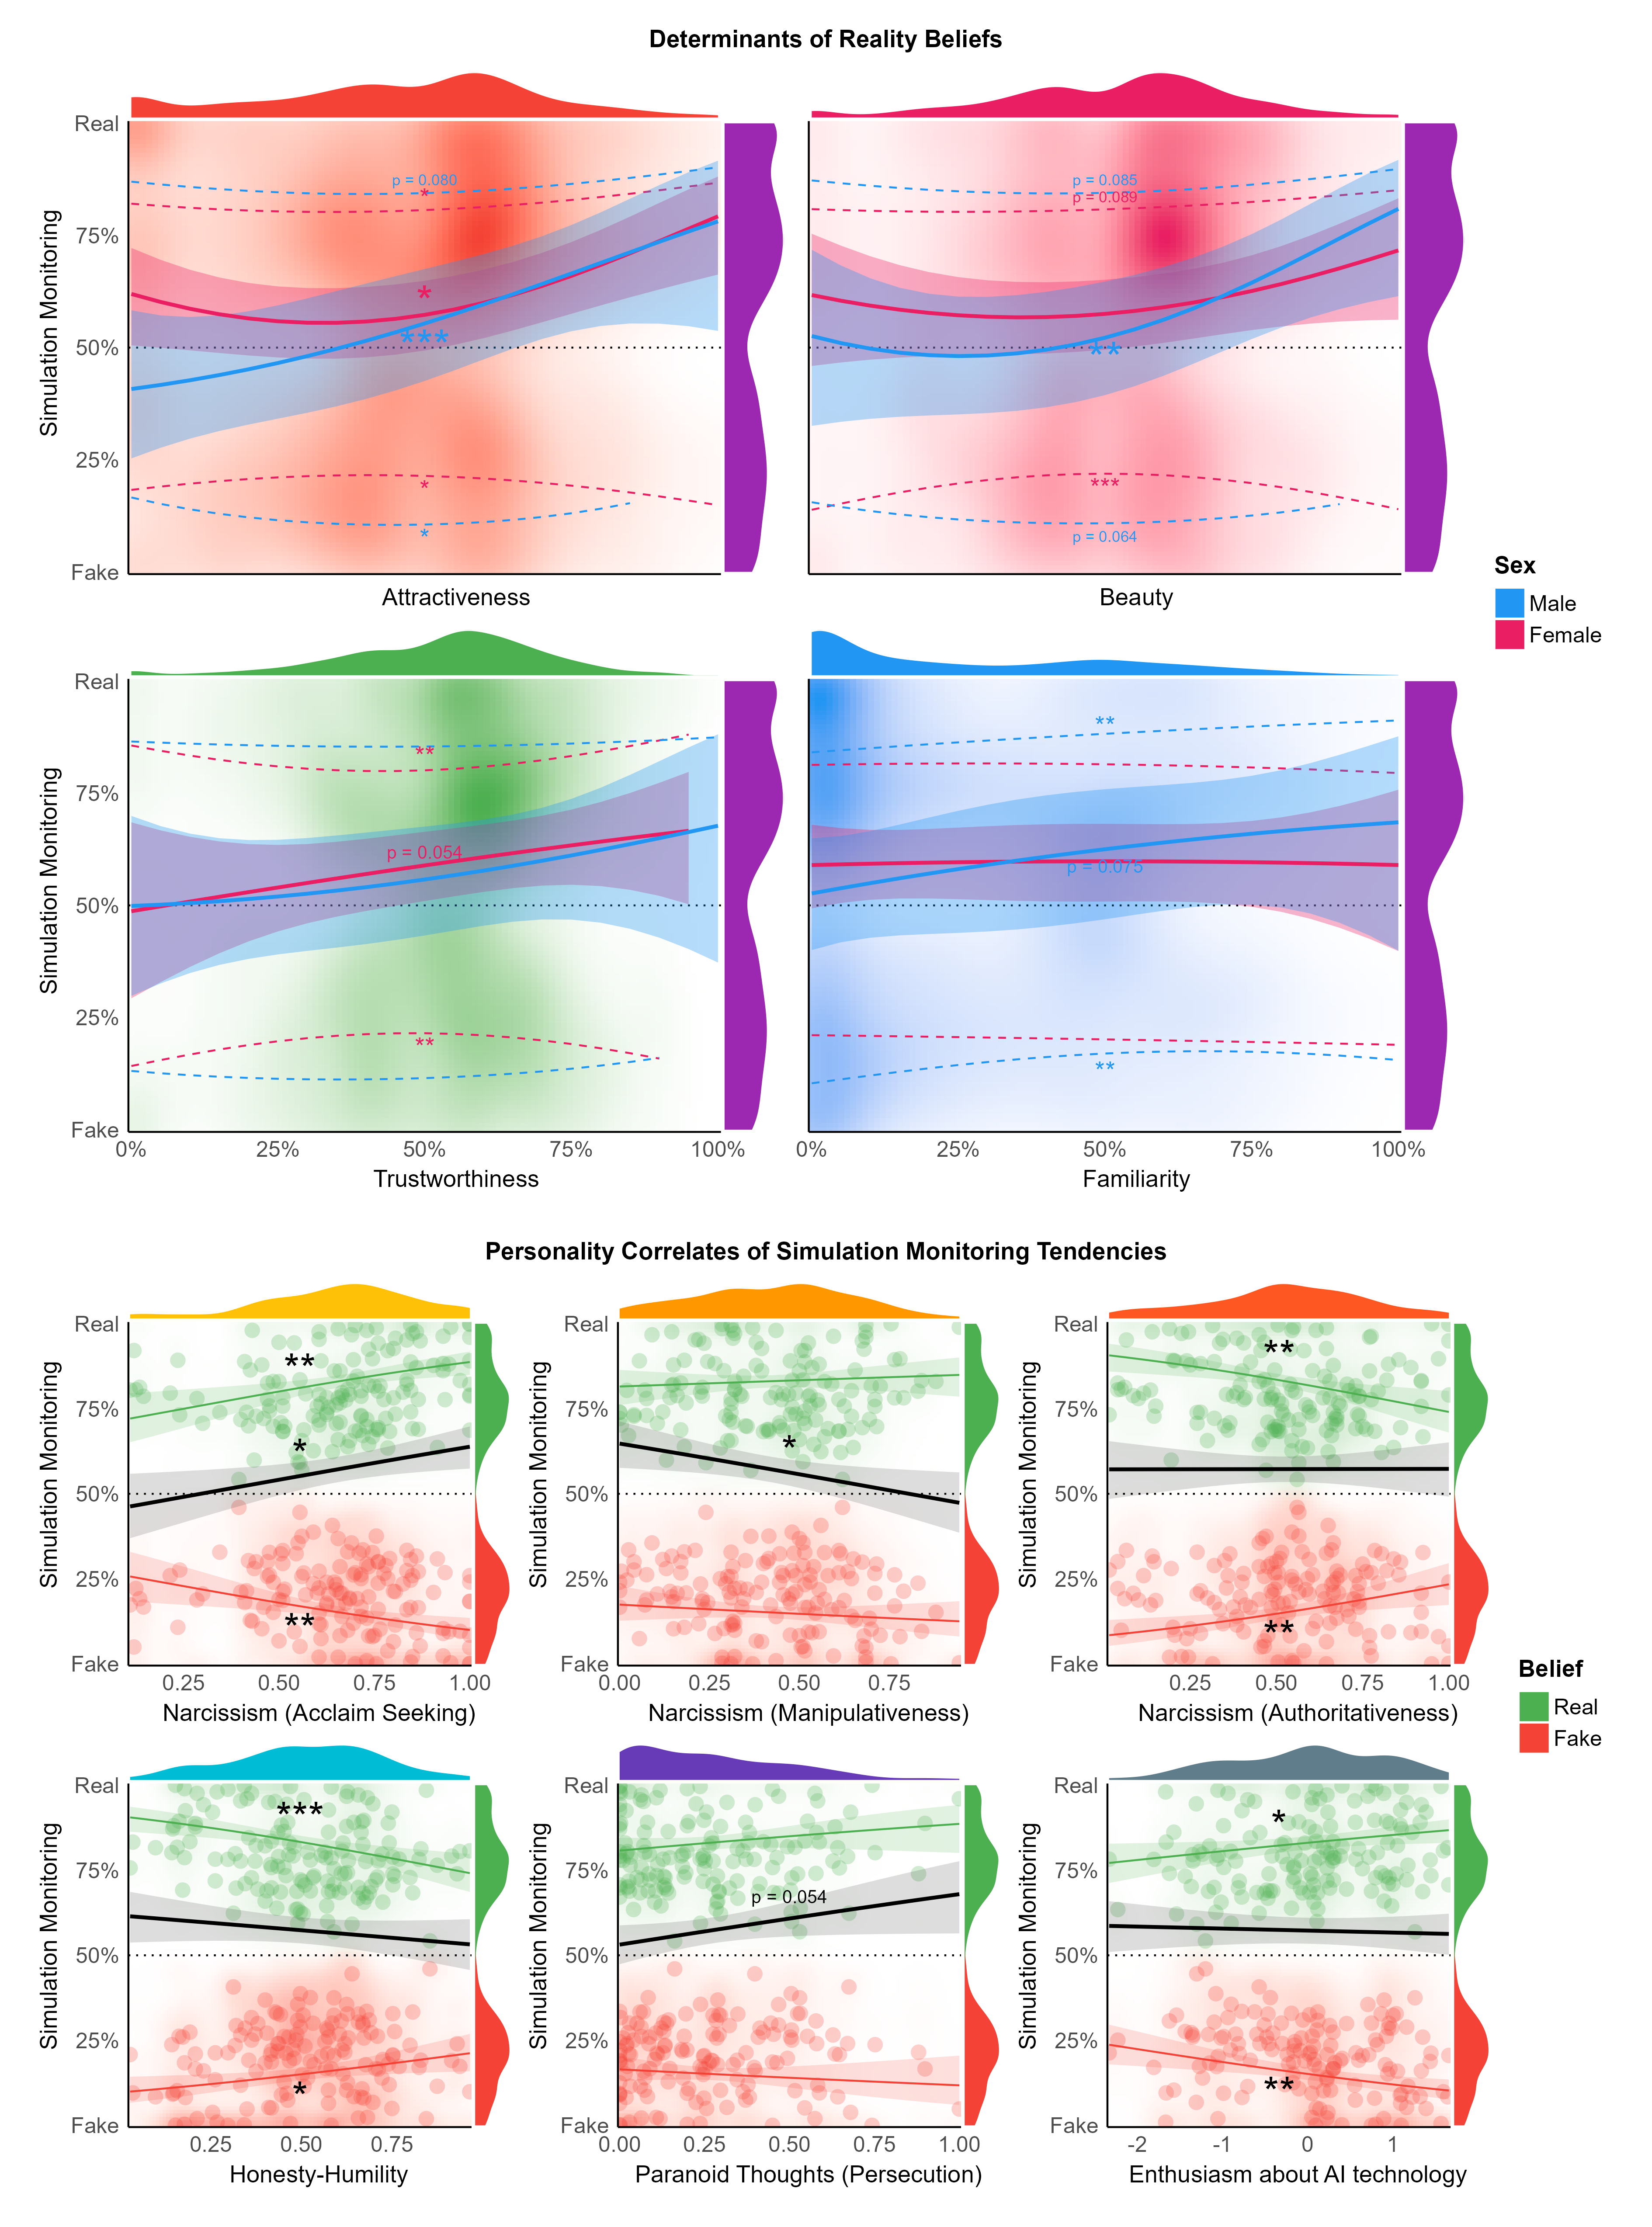
\includegraphics[width=1\linewidth]{../figures/Figure2} \caption{Top part shows the efffect of face ratings on 1) the probability of judging a face as real vs. fake (solid line) and 2) on the confidence associated with that judgement (dashed lines) depending on the sex. Bottom part shows the effect of personality traits on the belief (black line) and the confidence associated with it (colored lines). The points are the average per participant confidence for both types of judgements. Stars indicate significance (p < .001***, p < .01**, p < .05*).}\label{fig:unnamed-chunk-3}
\end{figure}

The analysis was carried out using \emph{R 4.2} (R Core Team, 2022), the \emph{tidyverse} (Wickham et al., 2019), and the \emph{easystats} collection of packages (Lüdecke et al., 2021, 2019, 2020; Makowski et al., 2020; Makowski, Ben-Shachar, et al., 2019). As all the details, scripts and complimentary analyses are open-access, we will focus in the manuscript on findings that are highly statistically significant (\(p <.01\)).

\hypertarget{results}{%
\subsection{Results}\label{results}}

\hypertarget{manipulation-check}{%
\subsubsection{Manipulation Check}\label{manipulation-check}}

Only one image file yielded a strong simulation monitoring bias (\textgreater{} 85\%), being classified as fake by 88.7\% of participants. This image was removed from further analysis, leaving 108 trials per participant. On average, across participants, 44\% of images (95\%\textasciitilde CI {[}0.12, 0.64{]}) were judged as fake and 56\% of images (95\%\textasciitilde CI {[}0.36, 0.84{]}) as real. An intercept-only model with the participants and images as random factors showed that the Intraclass Correlation Coefficient (ICC), which can be interpreted as the proportion of variance explained by the random factors, was of 9.0\% for the participants and 9.6\% for the stimuli.

While the delay of stimulus re-exposure stimulus did not have a significant effect on participants' beliefs of reality (\(OR = 1.00\), \(95\%~CI = [0.99, 1.00]\) ), judgement confidence was found to be negatively associated with re-exposure delay when the faces were judged as real (\(\beta = -0.006\), \(95\%~CI = [-0.1, 0.002]\), \(p = .004\))

\hypertarget{determinants-of-simulation-monitoring}{%
\subsubsection{Determinants of Simulation Monitoring}\label{determinants-of-simulation-monitoring}}

Attractiveness had a significant positive and linear relationship (\(R^2_{marginal}\) = 2.0\%) with the belief that a stimulus was real (\(\beta_{poly1} = 16.57\), \(95\%~CI = [7.33, 25.82]\), \(z = 3.51\), \(p < .001\)) for males, and a quadratic relationship for females (\(\beta_{poly2} = 7.82\), \(95\%~CI = [1.81, 13.84]\), \(z = 2.55\), \(p = .011\)), with both non-attractive and attractive faces being judged as more real. Attractiveness was also found to have a significant positive and quadratic relationship with confidence in judging faces both as real (\(\beta_{poly2} = 4.30\), \(95\%~CI = [0.97, 7.64]\), \(z = 2.53\), \(p = .011\)) and as fake (\(\beta_{poly2} = 5.23\), \(95\%~CI = [0. 86, 9.60]\), \(z = 2.35\), \(p = .019\)) for females. For males, however, a significant negative and quadratic relationship was found between attractiveness ratings and belief confidence only for faces judged as fake (\(\beta_{poly2} = -9.92\), \(95\%~CI = [-18.99, -0.86]\), \(z = -2.15\), \(p = .032\)). There was no interaction with reported self-attractiveness.

Beauty, adjusted for trustworthiness and familiarity, had a significant positive and linear relationship (\(R^2_{marginal}\) = 2.0\%) with the belief that a stimulus was real (\(\beta_{poly1} = 11.82\), \(95\%~CI = [4.28, 20.21]\), \(z = 2.76\), \(p = .006\)) for males only. No effect on confidence was found, aside from a quadratic relationship in females for faces judged as fake, suggesting that non-beautiful and highly beautiful faces were rated as fake with more confidence than average faces (\(\beta_{poly2} = 7.84\), \(95\%~CI = [3.39, 12.29]\), \(z = 3.46\), \(p < .001\)). There was no interaction with reported self-attractiveness.

Trustworthiness, adjusted for beauty and familiarity, had a predominantly positive and linear relationship (\(R^2_{marginal}\) = 2.0\%) with the belief that a stimulus was real (\(\beta_{poly1} = 6.44\), \(95\%~CI = [-0.11, 13.00]\), \(z = 1.93\), \(p = .0054\)) for females only. No effect on confidence was found for males, whereas a quadratic relationship was found for females for both faces judged as real (\(\beta_{poly2} = 6.14\), \(95\%~CI = [2.13, 10.14]\), \(z = 3.00\), \(p = .003\)) as well as fake (\(\beta_{poly2} =6.12\), \(95\%~CI = [1.49, 10.75]\), \(z = 2.59\), \(p = .001\)), suggesting that non-trustworthy and highly trustworthy faces were rated with more confidence than average faces.

We did not find any significant relationships for familiarity adjusted for beauty and trustworthiness (\(R^2_{marginal}\) = 2.0\%). However, a significant positive and linear relationship was found between familiarity and the confidence judgements of rating faces as real (\(\beta_{poly1} = 9.98\), \(95\%~CI = [3.83, 16.13]\), \(z = 3.18\), \(p = .001\)) whereas a negative linear relationship was found with those judged as fake (\(\beta_{poly1} = -12.41\), \(95\%~CI = [-20.27, -4.54]\), \(z = -3.09\), \(p = .002\)) for males only. This hence suggests that males more confidently judge faces as real with when they are familiar, and as fake when they are unfamiliar.

\hypertarget{inter-individual-correlates-of-simulation-monitoring}{%
\subsubsection{Inter-Individual Correlates of Simulation Monitoring}\label{inter-individual-correlates-of-simulation-monitoring}}

The models including the personality traits suggested that \emph{Honesty-Humility} had a significant negative relationship with the confidence associated with real as well as fake judgements (\(\beta_{real} = -1.62\), \(95\%~CI = [-2.55, -0.70]\), \(z = -3.43\), \(p < .001\); \(\beta_{fake} = -1.16\), \(95\%~CI = [-2.09, -0.23]\), \(z = -2.45\), \(p = 0.014\)).

Significant positive associations were found between the probability of judging faces as real and dimensions of narcissism such as \emph{Acclaim Seeking} (\(\beta = 2.24\), \(95\%~CI = [1.17, 4.27]\), \(z = 2.44\), \(p = .015\)), and \emph{Manipulativeness} (\(\beta = 0.47\), \(95\%~CI = [0.25, 0.87]\), \(z = -2.4\), \(p = 0.017\)). Confidence judgements also shared significant links with narcissism through various facets, such as a positive relationship between the confidence for both real and fake judgements with \emph{Acclaim Seeking} (\(\beta_{real} = 1.65\), \(95\%~CI = [0.59, 2.70]\), \(z = 3.07\), \(p =.002\); \(\beta_{fake} = 1.62\), \(95\%~CI = [0.56, 2.68]\), \(z = 3.00\), \(p = .003\)), and a negative relationship with \emph{Authoritativeness} (\(\beta_{real} = -1.57\), \(95\%~CI = [-2.58, -0.57]\), \(z = -3.08\), \(p = .002\); \(\beta_{fake} = -1.49\), \(95\%~CI = [-2.50, -0.48]\), \(z = -2.89\), \(p = .004\)).

A positive trend was found in the relationship between the \emph{Persecutory Ideation} dimension of paranoid thinking and the belief that the faces were real (\(\beta = 1.87\), \(95\%~CI = [0.99, 3.54]\), \(z = 1.93\), \(p = .054\)).

The \emph{Prospective Anxiety} aspect of intolerance to uncertainty shared a negative trend in its association with confidence ratings (\(\beta_{real} = 1.43\), \(95\%~CI = [0.10, 2.76]\), \(z = 2.10\), \(p = .036\); \(\beta_{fake} = -0.91\), \(95\%~CI = [-1.93, 0.11]\), \(z = -1.75\), \(p = .081\)). No significant effect was found for social anxiety.

Questions pertaining to the attitude towards AI were reduced to 3 dimensions through factor analysis, labelled AI-Enthusiasm (loaded by items expressing interest and excitement in AI development and applications), AI-Realness (loaded by items expressing positive opinions on the ability of AI to create realistic material), and AI-Danger (loaded by items expressing concerns on the unethical misuse of AI technology). However, only AI-Enthusiasm displayed a significant positive relationship with the confidence in both real and fake judgements (\(\beta_{real} = 0.21\), \(95\%~CI = [0.02, 0.40]\), \(z = 2.20\), \(p = .028\); \(\beta_{fake} = 0.31\), \(95\%~CI = [0.12, 0.50]\), \(z = -8.90\), \(p < 0.001\)).

\hypertarget{discussion}{%
\subsection{Discussion}\label{discussion}}

This study aimed at investigating the effect of facial ratings (attractiveness, beauty, trustworthiness and familiarity) on simulation monitoring, i.e., on the belief that a stimulus was artificially generated. Most strikingly, despite all the stimuli being real faces from the same database, all participants believed (to high degrees of confidence) that a significant proportion of them were fake. This finding not only attests to the effectiveness of our instructions, but highlights the current levels of expectation regarding CGI technology. The strong impact of prior expectations and information on reality beliefs demonstrated here underlines the volatility of our sense of reality. In fact, stimuli-related and participant-related characteristics accounted together for less than 20\% of the beliefs variance, suggesting a large contribution of other subjective processes.

Although attractiveness did not seem to be the primary drive underlying simulation monitoring of face images, we do nonetheless report significant associations, with a different pattern observed depending on the participant's gender. The quadratic relationship found for female participants is aligned with our hypothesis that salient faces (i.e., rated as very attractive or very unattractive) are judged to be more real. The fact that this effect did not reach significance for beauty underlines that attractiveness judgement, and its role in simulation monitoring, is a multidimensional construct that cannot be reduced to physical facial attractiveness, in particular for women (Buunk et al., 2002; Qi \& Ying, 2022). In fact, female participants were more confident in judging faces as fake only when they were rated very high or low on beauty, suggesting that physical beauty and attractiveness are not analogous in their effects on simulation monitoring decisions.

Interestingly, we found a significant positive linear relationship in male participants for both attractiveness and beauty on simulation monitoring that we could interpret under an evolutionary lens. Specifically, males purportedly place more emphasis on facial attractiveness as a sign of reproductive potential, as compared with females, who tend to value characteristics signaling resource acquisition capabilities (Buunk et al., 2002; Fink et al., 2006; Qi \& Ying, 2022). It is thus possible that the evolutionary weight associated with attractiveness skewed the perceived saliency of men towards attractive faces, rendering them significantly more salient than unattractive faces, and in turn distorted the relationship with simulation monitoring. However, future studies should test this saliency-based hypothesis by measuring constructs closer to salience and its effects, for instance using neuroimaging (Indovina \& Macaluso, 2007; Lou et al., 2015) or physiological markers
(e.g., heart rate deceleration, Skora et al., 2022).

Our results found a positive linear trend between trustworthiness and simulation monitoring for females only. Given prior evidence that faces presented as computer-generated were rated less trustworthy (Balas \& Pacella, 2017; Hoogers, 2021; Liefooghe et al., 2022), we expected such a linear association to be more clearly present for both genders. One of the underlying mechanisms that possibly contributed to this dimorphism could be the increased risk-taking aversion reported in females
(explained evolutionarily as a compromise to their reproductive potential, Van Den Akker et al., 2020),
to which perceived facial trustworthiness relates (Hou \& Liu, 2019). However, if that was the case, faces judged as highly untrustworthy should have appeared as even more salient (representing an evolutionary threat), and hence be judged as more real, leading to a quadratic relationship between trustworthiness and simulation monitoring instead. Further studies are needed to investigate the causes of the increased simulation monitoring sensitivity to trustworthiness in females.

Contrary to our hypothesis, we did not find familiarity to be significantly related to simulation monitoring decisions. Interestingly, there were significant linear relationships between familiarity and confidence judgements for males only, where familiarity increased the confidence of reality beliefs. Although the familiarity measure was not a ``recognition'' measure, evidence from studies pertaining to the latter could be linked, reporting better face memory for females (Lewin \& Herlitz, 2002; Mishra et al., 2019; Sommer et al., 2013), as well as an overconfidence in face recall for males (Bailey, 2021; Herbst, 2020). However, it should be noted that the present study's distribution of familiarity ratings was strongly skewed, and only a low number of pictures was rated as highly familiar. As such, future studies should clarify this point by experimentally manipulating familiarity, for instance by modulating the amount of exposure to items before querying the simulation monitoring judgements.

Regarding the role of inter-individual characteristics in simulation monitoring tendencies, we found higher scores of honesty-humility - a trait related to an increased risk perception and aversion (Levidi et al., 2022; Weller \& Thulin, 2012) - to be related to a lower confidence in simulation monitoring judgements. Notably, greater narcissistic tendencies in dimensions such as acclaim seeking and manipulativeness were associated with a higher number of faces judged as real. This is in line with recent research which found people with narcissism to be less likely to engage in analytical reasoning strategies such as reflective thinking (Ahadzadeh et al., 2021; Littrell et al., 2020), and to be more vigilant and attentive to external stimuli (Carolan, 2017; Eddy, 2021; Grapsas et al., 2020).

Moreover, putting the significant positive links between narcissistic acclaim seeking and confidence judgements in perspective with the negative correlation between honesty-humility and narcissism (Hodson et al., 2018), we confirm previous evidence regarding the relationship between narcissistic grandiosity and over-confidence in decision-making (Brunell \& Buelow, 2017; Campbell et al., 2004; Chatterjee \& Pollock, 2017; O'Reilly \& Hall, 2021). Although an inverse effect was found for the narcissistic facet of authoritativeness, we interpret this relationship as related to a higher response assertiveness. Taken together, these results suggest that participants with low humility and high recognition desires are more confident in their judgement regarding the real or fake nature of ambiguous stimuli. Alternatively, participants with opposite traits might perceive a higher risk in the decision-making process and its potential consequences (e.g., being seen as bad at the task at hand), resulting in more conservative confidence ratings.

Our findings suggest - though with weak significance - a positive link between paranoid ideation and the tendency to believe that the stimuli were real. Given previous reports that people with higher levels of paranoia are more sensitive to cues of social threat (Fornells-Ambrojo et al., 2015; Freeman et al., 2003; King \& Dudley, 2017), it is plausible that paranoid traits confer greater saliency and emotionality to observed faces, hence increasing perceptions of its realness. This hypothesis, if confirmed by future studies, would be in line with previous findings that persecutory delusions are predicted by a greater sense of presence in VR environments populated with virtual characters (Freeman et al., 2005).

Despite the ubiquity of AI, the literature pertaining to the influence of people's AI attitudes on simulation monitoring is scarce. Contrary to our expectations, we did not find evidence for the role of participants' expectations regarding the capabilities of AI technology (in terms of the realism of its productions). Instead, we found only one's enthusiasm about AI technology to be related to an increased confidence in simulation monitoring ratings. This could potentially be because participants with a highly positive attitude towards AI perceive themselves as having greater knowledge about AI and its capabilities (Said et al., 2022), hence permitting themselves to be more confident in their simulation monitoring decisions. In fact, this result is in line with reports that AI attitudes interacts with people's perceived self-knowledge to influence their perception of the opportunities and risks accorded by AI applications (Said et al., 2022).

On a methodological level, although the order of presentation of the facial images was randomized to reduce effects of adaptation, participants were more confident in their judgements for faces perceived as real following a shorter re-exposure delay. Such shorter durations could be associated with the faces being better remembered and appearing more familiar, thereby triggering self-referential and autobiographical memory processing during the repeated display (Abraham \& Von Cramon, 2009; Gobbini et al., 2013; Taylor et al., 2009). Indeed, this finding is consistent with studies in which fictional stimuli that were associated with familiarity up-regulated emotions, biasing its salience and perceived realness (Makowski et al., 2017; Sperduti et al., 2016). However, if that was the case, we would expect shorter re-exposure delays to impact the decision bias as well towards reality, rather than simply the confidence. Future studies should further investigate the modulatory effects of types and degrees of familiarity on perceived realness judgements.

Several limitations have to be noted. The current experimental paradigm required participants to judge the realness of faces they had prior exposure to (which was done to prevent reality judgements from influencing the other ratings). Although the effect of re-exposure delay was negligible, the potential bias induced by face familiarity (as compared to judging completely new items) cannot be discarded. Future studies could examine that by incorporating novel face images or increasing the duration of the re-exposure delay. Moreover, the magnitude of the effects found in the study was relatively small, suggesting that the facial features measured in the study were not the key determinants of simulation monitoring. Hence, beyond exploring new potential mechanisms, future studies should include a more thorough debriefing to try to capture what conscious strategies (if any) the participants used (e.g., focusing on some features of the stimulus - like hair or eyes in the case of faces) to guide their reality beliefs.

In summary, the aim of the present study was to examine whether a subset of specific characteristics, in particular face attractiveness, significantly influences our simulation monitoring decisions. Notably, we found faces rated as attractive to be perceived as more real, with a possible sexual dimorphism affecting the shape of the relationship. We also found that inter-individual traits, such as narcissistic acclaim-seeking and manipulativeness, as well as persecutory ideation, were related to a systematic bias towards beliefs that the stimuli were real or fake. We believe that these findings provide the foundations to help us understand what drives reality beliefs in an increasingly reality-ambiguous world.

\hypertarget{data-availability}{%
\section{Data Availability}\label{data-availability}}

The datasets generated and/or analysed during the current study are available in the GitHub repository \url{https://github.com/RealityBending/FakeFace}

\hypertarget{funding}{%
\section{Funding}\label{funding}}

This work was supported by the Presidential Postdoctoral Fellowship Grant (NTU-PPF-2020-10014) from Nanyang Technological University (awarded to DM) and the Intra-CREATE Seed Collaboration Grant (NRF2021-ITS008-0010) from the National Research Foundation, Prime Minister's Office, Singapore, under its Campus for Research Excellence and Technological Enterprise (CREATE) programme (awarded to DM and PM).

\hypertarget{acknowledgments}{%
\section{Acknowledgments}\label{acknowledgments}}

We would like to thank Taong Ren Qing Malcolm for his contribution to the selection of the materials.

\newpage

\hypertarget{references}{%
\section{References}\label{references}}

\hypertarget{refs}{}
\begin{CSLReferences}{1}{0}
\leavevmode\vadjust pre{\hypertarget{ref-abraham2009reality}{}}%
Abraham, A., \& Von Cramon, D. Y. (2009). Reality= relevance? Insights from spontaneous modulations of the brain's default network when telling apart reality from fiction. \emph{PloS One}, \emph{4}(3), e4741.

\leavevmode\vadjust pre{\hypertarget{ref-ahadzadeh2021social}{}}%
Ahadzadeh, A. S., Ong, F. S., \& Wu, S. L. (2021). Social media skepticism and belief in conspiracy theories about COVID-19: The moderating role of the dark triad. \emph{Current Psychology}, 1--13.

\leavevmode\vadjust pre{\hypertarget{ref-bago2022emotion}{}}%
Bago, B., Rosenzweig, L. R., Berinsky, A. J., \& Rand, D. G. (2022). Emotion may predict susceptibility to fake news but emotion regulation does not seem to help. \emph{Cognition and Emotion}, 1--15.

\leavevmode\vadjust pre{\hypertarget{ref-bailey2021gender}{}}%
Bailey, A. (2021). \emph{A gender in-group effect on facial recall} {[}PhD thesis{]}. University of Tasmania.

\leavevmode\vadjust pre{\hypertarget{ref-balas2017}{}}%
Balas, B., \& Pacella, J. (2017). Trustworthiness perception is disrupted in artificial faces. \emph{Computers in Human Behavior}, \emph{77}. \url{https://doi.org/10.1016/j.chb.2017.08.045}

\leavevmode\vadjust pre{\hypertarget{ref-bartosik2021you}{}}%
Bartosik, B., Wojcik, G. M., Brzezicka, A., \& Kawiak, A. (2021). Are you able to trust me? Analysis of the relationships between personality traits and the assessment of attractiveness and trust. \emph{Frontiers in Human Neuroscience}, \emph{15}, 685530.

\leavevmode\vadjust pre{\hypertarget{ref-begg1992dissociation}{}}%
Begg, I. M., Anas, A., \& Farinacci, S. (1992). Dissociation of processes in belief: Source recollection, statement familiarity, and the illusion of truth. \emph{Journal of Experimental Psychology: General}, \emph{121}(4), 446.

\leavevmode\vadjust pre{\hypertarget{ref-berghel2018weaponizing}{}}%
Berghel, H. (2018). Weaponizing twitter litter: Abuse-forming networks and social media. \emph{Computer}, \emph{51}(4), 70--73.

\leavevmode\vadjust pre{\hypertarget{ref-britt2019reasoned}{}}%
Britt, M. A., Rouet, J.-F., Blaum, D., \& Millis, K. (2019). A reasoned approach to dealing with fake news. \emph{Policy Insights from the Behavioral and Brain Sciences}, \emph{6}(1), 94--101.

\leavevmode\vadjust pre{\hypertarget{ref-brunell2017narcissism}{}}%
Brunell, A. B., \& Buelow, M. T. (2017). Narcissism and performance on behavioral decision-making tasks. \emph{Journal of Behavioral Decision Making}, \emph{30}(1), 3--14.

\leavevmode\vadjust pre{\hypertarget{ref-bryanov2021determinants}{}}%
Bryanov, K., \& Vziatysheva, V. (2021). Determinants of individuals' belief in fake news: A scoping review determinants of belief in fake news. \emph{PLoS One}, \emph{16}(6), e0253717.

\leavevmode\vadjust pre{\hypertarget{ref-buunk2002age}{}}%
Buunk, B. P., Dijkstra, P., Fetchenhauer, D., \& Kenrick, D. T. (2002). Age and gender differences in mate selection criteria for various involvement levels. \emph{Personal Relationships}, \emph{9}(3), 271--278.

\leavevmode\vadjust pre{\hypertarget{ref-calbi2017}{}}%
Calbi, M., Heimann, K., Barratt, D., Siri, F., Umiltà, M. A., \& Gallese, V. (2017). How context influences our perception of emotional faces: A behavioral study on the kuleshov effect. \emph{Frontiers in Psychology}, \emph{8}. \url{https://www.frontiersin.org/articles/10.3389/fpsyg.2017.01684}

\leavevmode\vadjust pre{\hypertarget{ref-campbell2004narcissism}{}}%
Campbell, W. K., Goodie, A. S., \& Foster, J. D. (2004). Narcissism, confidence, and risk attitude. \emph{Journal of Behavioral Decision Making}, \emph{17}(4), 297--311.

\leavevmode\vadjust pre{\hypertarget{ref-carleton2007fearing}{}}%
Carleton, R. N., Norton, M. P. J., \& Asmundson, G. J. (2007). Fearing the unknown: A short version of the intolerance of uncertainty scale. \emph{Journal of Anxiety Disorders}, \emph{21}(1), 105--117.

\leavevmode\vadjust pre{\hypertarget{ref-carolan2017searching}{}}%
Carolan, P. L. (2017). \emph{Searching {``inaffectively''}: A behavioral, psychometric, and electroencephalographic investigation of psychopathic personality and visual-spatial attention} {[}PhD thesis{]}. Arts \& Social Sciences: Department of Psychology.

\leavevmode\vadjust pre{\hypertarget{ref-chatterjee2017master}{}}%
Chatterjee, A., \& Pollock, T. G. (2017). Master of puppets: How narcissistic CEOs construct their professional worlds. \emph{Academy of Management Review}, \emph{42}(4), 703--725.

\leavevmode\vadjust pre{\hypertarget{ref-chen2021broadening}{}}%
Chen, J. M., Norman, J. B., \& Nam, Y. (2021). Broadening the stimulus set: Introducing the american multiracial faces database. \emph{Behavior Research Methods}, \emph{53}(1), 371--389.

\leavevmode\vadjust pre{\hypertarget{ref-chen2015news}{}}%
Chen, Y., Conroy, N. K., \& Rubin, V. L. (2015). News in an online world: The need for an {``automatic crap detector.''} \emph{Proceedings of the Association for Information Science and Technology}, \emph{52}(1), 1--4.

\leavevmode\vadjust pre{\hypertarget{ref-de2015jspsych}{}}%
De Leeuw, J. R. (2015). jsPsych: A JavaScript library for creating behavioral experiments in a web browser. \emph{Behavior Research Methods}, \emph{47}(1), 1--12.

\leavevmode\vadjust pre{\hypertarget{ref-ecker2022psychological}{}}%
Ecker, U. K., Lewandowsky, S., Cook, J., Schmid, P., Fazio, L. K., Brashier, N., Kendeou, P., Vraga, E. K., \& Amazeen, M. A. (2022). The psychological drivers of misinformation belief and its resistance to correction. \emph{Nature Reviews Psychology}, \emph{1}(1), 13--29.

\leavevmode\vadjust pre{\hypertarget{ref-eddy2021self}{}}%
Eddy, C. M. (2021). Self-serving social strategies: A systematic review of social cognition in narcissism. \emph{Current Psychology}, 1--19.

\leavevmode\vadjust pre{\hypertarget{ref-fink2006facial}{}}%
Fink, B., Neave, N., Manning, J. T., \& Grammer, K. (2006). Facial symmetry and judgements of attractiveness, health and personality. \emph{Personality and Individual Differences}, \emph{41}(3), 491--499.

\leavevmode\vadjust pre{\hypertarget{ref-fornells2015people}{}}%
Fornells-Ambrojo, M., Freeman, D., Slater, M., Swapp, D., Antley, A., \& Barker, C. (2015). How do people with persecutory delusions evaluate threat in a controlled social environment? A qualitative study using virtual reality. \emph{Behavioural and Cognitive Psychotherapy}, \emph{43}(1), 89--107.

\leavevmode\vadjust pre{\hypertarget{ref-freeman2005psychology}{}}%
Freeman, D., Garety, P. A., Bebbington, P., Slater, M., Kuipers, E., Fowler, D., Green, C., Jordan, J., Ray, K., \& Dunn, G. (2005). The psychology of persecutory ideation II: A virtual reality experimental study. \emph{The Journal of Nervous and Mental Disease}, \emph{193}(5), 309--315.

\leavevmode\vadjust pre{\hypertarget{ref-freeman2021revised}{}}%
Freeman, D., Loe, B. S., Kingdon, D., Startup, H., Molodynski, A., Rosebrock, L., Brown, P., Sheaves, B., Waite, F., \& Bird, J. C. (2021). The revised green et al., Paranoid thoughts scale (r-GPTS): Psychometric properties, severity ranges, and clinical cut-offs. \emph{Psychological Medicine}, \emph{51}(2), 244--253.

\leavevmode\vadjust pre{\hypertarget{ref-freeman2003can}{}}%
Freeman, D., Slater, M., Bebbington, P. E., Garety, P. A., Kuipers, E., Fowler, D., Met, A., Read, C. M., Jordan, J., \& Vinayagamoorthy, V. (2003). Can virtual reality be used to investigate persecutory ideation? \emph{The Journal of Nervous and Mental Disease}, \emph{191}(8), 509--514.

\leavevmode\vadjust pre{\hypertarget{ref-garrido2017kdef}{}}%
Garrido, M. V., \& Prada, M. (2017). KDEF-PT: Valence, emotional intensity, familiarity and attractiveness ratings of angry, neutral, and happy faces. \emph{Frontiers in Psychology}, \emph{8}, 2181.

\leavevmode\vadjust pre{\hypertarget{ref-gobbini2013prioritized}{}}%
Gobbini, M. I., Gors, J. D., Halchenko, Y. O., Rogers, C., Guntupalli, J. S., Hughes, H., \& Cipolli, C. (2013). Prioritized detection of personally familiar faces. \emph{PloS One}, \emph{8}(6), e66620.

\leavevmode\vadjust pre{\hypertarget{ref-goldstein2009pleasure}{}}%
Goldstein, T. R. (2009). The pleasure of unadulterated sadness: Experiencing sorrow in fiction, nonfiction, and" in person.". \emph{Psychology of Aesthetics, Creativity, and the Arts}, \emph{3}(4), 232.

\leavevmode\vadjust pre{\hypertarget{ref-grapsas2020and}{}}%
Grapsas, S., Brummelman, E., Back, M. D., \& Denissen, J. J. (2020). The {``why''} and {``how''} of narcissism: A process model of narcissistic status pursuit. \emph{Perspectives on Psychological Science}, \emph{15}(1), 150--172.

\leavevmode\vadjust pre{\hypertarget{ref-han2018beauty}{}}%
Han, S., Li, Y., Liu, S., Xu, Q., Tan, Q., \& Zhang, L. (2018). Beauty is in the eye of the beholder: The halo effect and generalization effect in the facial attractiveness evaluation. \emph{Acta Psychologica Sinica}, \emph{50}(4), 363.

\leavevmode\vadjust pre{\hypertarget{ref-herbst2020gender}{}}%
Herbst, T. H. (2020). Gender differences in self-perception accuracy: The confidence gap and women leaders' underrepresentation in academia. \emph{SA Journal of Industrial Psychology}, \emph{46}(1), 1--8.

\leavevmode\vadjust pre{\hypertarget{ref-hodson2018dark}{}}%
Hodson, G., Book, A., Visser, B. A., Volk, A. A., Ashton, M. C., \& Lee, K. (2018). Is the dark triad common factor distinct from low honesty-humility? \emph{Journal of Research in Personality}, \emph{73}, 123--129.

\leavevmode\vadjust pre{\hypertarget{ref-hoogers2021effect}{}}%
Hoogers, E. (2021). \emph{The effect of attitude towards computer generated faces on face perception} {[}\{B.S.\} thesis{]}.

\leavevmode\vadjust pre{\hypertarget{ref-hou2019survival}{}}%
Hou, C., \& Liu, Z. (2019). The survival processing advantage of face: The memorization of the (un) trustworthy face contributes more to survival adaptation. \emph{Evolutionary Psychology}, \emph{17}(2), 1474704919839726.

\leavevmode\vadjust pre{\hypertarget{ref-indovina2007dissociation}{}}%
Indovina, I., \& Macaluso, E. (2007). Dissociation of stimulus relevance and saliency factors during shifts of visuospatial attention. \emph{Cerebral Cortex}, \emph{17}(7), 1701--1711.

\leavevmode\vadjust pre{\hypertarget{ref-jauk2022validation}{}}%
Jauk, E., Olaru, G., Schürch, E., Back, M. D., \& Morf, C. C. (2022). Validation of the german five-factor narcissism inventory and construction of a brief form using ant colony optimization. \emph{Assessment}, 10731911221075761.

\leavevmode\vadjust pre{\hypertarget{ref-king2017paranoia}{}}%
King, A., \& Dudley, R. (2017). Paranoia, worry, cognitive avoidance and intolerance of uncertainty in a student population. \emph{Journal of Applied Psychology and Social Science}, \emph{3}(2), 70--89.

\leavevmode\vadjust pre{\hypertarget{ref-levidi2022understanding}{}}%
Levidi, M. D. C., McGrath, A., Kyriakoulis, P., \& Sulikowski, D. (2022). Understanding criminal decision-making: Links between honesty-humility, perceived risk and negative affect: Psychology, crime \& law. \emph{Psychology, Crime and Law}, 1--29.

\leavevmode\vadjust pre{\hypertarget{ref-lewandowsky2017beyond}{}}%
Lewandowsky, S., Ecker, U. K., \& Cook, J. (2017). Beyond misinformation: Understanding and coping with the {``post-truth''} era. \emph{Journal of Applied Research in Memory and Cognition}, \emph{6}(4), 353--369.

\leavevmode\vadjust pre{\hypertarget{ref-lewin2002sex}{}}%
Lewin, C., \& Herlitz, A. (2002). Sex differences in face recognition---women's faces make the difference. \emph{Brain and Cognition}, \emph{50}(1), 121--128.

\leavevmode\vadjust pre{\hypertarget{ref-liefooghe2022faces}{}}%
Liefooghe, B., Oliveira, M., Leisten, L. M., Hoogers, E., Aarts, H., \& Hortensius, R. (2022). \emph{Faces merely labelled as artificial are trusted less}.

\leavevmode\vadjust pre{\hypertarget{ref-little2011facial}{}}%
Little, A. C., Jones, B. C., \& DeBruine, L. M. (2011). Facial attractiveness: Evolutionary based research. \emph{Philosophical Transactions of the Royal Society B: Biological Sciences}, \emph{366}(1571), 1638--1659.

\leavevmode\vadjust pre{\hypertarget{ref-littrell2020overconfidently}{}}%
Littrell, S., Fugelsang, J., \& Risko, E. F. (2020). Overconfidently underthinking: Narcissism negatively predicts cognitive reflection. \emph{Thinking \& Reasoning}, \emph{26}(3), 352--380.

\leavevmode\vadjust pre{\hypertarget{ref-lou2015perceptual}{}}%
Lou, B., Hsu, W.-Y., \& Sajda, P. (2015). Perceptual salience and reward both influence feedback-related neural activity arising from choice. \emph{Journal of Neuroscience}, \emph{35}(38), 13064--13075.

\leavevmode\vadjust pre{\hypertarget{ref-parametersArticle}{}}%
Lüdecke, D., Ben-Shachar, M., Patil, I., \& Makowski, D. (2020). Extracting, computing and exploring the parameters of statistical models using {R}. \emph{Journal of Open Source Software}, \emph{5}(53), 2445. \url{https://doi.org/10.21105/joss.02445}

\leavevmode\vadjust pre{\hypertarget{ref-performanceArticle}{}}%
Lüdecke, D., Ben-Shachar, M., Patil, I., Waggoner, P., \& Makowski, D. (2021). {performance}: An {R} package for assessment, comparison and testing of statistical models. \emph{Journal of Open Source Software}, \emph{6}(60), 3139. \url{https://doi.org/10.21105/joss.03139}

\leavevmode\vadjust pre{\hypertarget{ref-insightArticle}{}}%
Lüdecke, D., Waggoner, P., \& Makowski, D. (2019). Insight: A unified interface to access information from model objects in {R}. \emph{Journal of Open Source Software}, \emph{4}(38), 1412. \url{https://doi.org/10.21105/joss.01412}

\leavevmode\vadjust pre{\hypertarget{ref-makowski2018cognitive}{}}%
Makowski, D. (2018). \emph{Cognitive neuropsychology of implicit emotion regulation through fictional reappraisal} {[}PhD thesis{]}. Sorbonne Paris Cit{é}.

\leavevmode\vadjust pre{\hypertarget{ref-bayestestRArticle}{}}%
Makowski, D., Ben-Shachar, M., \& Lüdecke, D. (2019). {bayestestR}: Describing effects and their uncertainty, existence and significance within the {Bayesian} framework. \emph{Journal of Open Source Software}, \emph{4}(40), 1541. \url{https://doi.org/10.21105/joss.01541}

\leavevmode\vadjust pre{\hypertarget{ref-correlationArticle}{}}%
Makowski, D., Ben-Shachar, M., Patil, I., \& Lüdecke, D. (2020). Methods and algorithms for correlation analysis in {R}. \emph{Journal of Open Source Software}, \emph{5}(51), 2306. \url{https://doi.org/10.21105/joss.02306}

\leavevmode\vadjust pre{\hypertarget{ref-makowski2017being}{}}%
Makowski, D., Sperduti, M., Nicolas, S., \& Piolino, P. (2017). {``Being there''} and remembering it: Presence improves memory encoding. \emph{Consciousness and Cognition}, \emph{53}, 194--202.

\leavevmode\vadjust pre{\hypertarget{ref-makowski2019phenomenal}{}}%
Makowski, D., Sperduti, M., Pelletier, J., Blondé, P., La Corte, V., Arcangeli, M., Zalla, T., Lemaire, S., Dokic, J., Nicolas, S., et al. (2019). Phenomenal, bodily and brain correlates of fictional reappraisal as an implicit emotion regulation strategy. \emph{Cognitive, Affective, \& Behavioral Neuroscience}, \emph{19}(4), 877--897.

\leavevmode\vadjust pre{\hypertarget{ref-marcinkowska2021self}{}}%
Marcinkowska, U. M., Jones, B. C., \& Lee, A. J. (2021). Self-rated attractiveness predicts preferences for sexually dimorphic facial characteristics in a culturally diverse sample. \emph{Scientific Reports}, \emph{11}(1), 1--8.

\leavevmode\vadjust pre{\hypertarget{ref-martel2020reliance}{}}%
Martel, C., Pennycook, G., \& Rand, D. G. (2020). Reliance on emotion promotes belief in fake news. \emph{Cognitive Research: Principles and Implications}, \emph{5}(1), 1--20.

\leavevmode\vadjust pre{\hypertarget{ref-mcdonnell2010face}{}}%
McDonnell, R., \& Breidt, M. (2010). Face reality: Investigating the uncanny valley for virtual faces. In \emph{ACM SIGGRAPH ASIA 2010 sketches} (pp. 1--2).

\leavevmode\vadjust pre{\hypertarget{ref-michael2021source}{}}%
Michael, R. B., \& Sanson, M. (2021). Source information affects interpretations of the news across multiple age groups in the united states. \emph{Societies}, \emph{11}(4), 119.

\leavevmode\vadjust pre{\hypertarget{ref-mishra2019gender}{}}%
Mishra, M. V., Likitlersuang, J., B Wilmer, J., Cohan, S., Germine, L., \& DeGutis, J. M. (2019). Gender differences in familiar face recognition and the influence of sociocultural gender inequality. \emph{Scientific Reports}, \emph{9}(1), 1--12.

\leavevmode\vadjust pre{\hypertarget{ref-moshel2022}{}}%
Moshel, M. L., Robinson, A. K., Carlson, T. A., \& Grootswagers, T. (2022). Are you for real? Decoding realistic AI-generated faces from neural activity. \emph{Vision Research}, \emph{199}, 108079. \url{https://doi.org/10.1016/j.visres.2022.108079}

\leavevmode\vadjust pre{\hypertarget{ref-nightingale2022}{}}%
Nightingale, S. J., \& Farid, H. (2022). AI-synthesized faces are indistinguishable from real faces and more trustworthy. \emph{Proceedings of the National Academy of Sciences}, \emph{119}(8), e2120481119. \url{https://doi.org/10.1073/pnas.2120481119}

\leavevmode\vadjust pre{\hypertarget{ref-o2021grandiose}{}}%
O'Reilly, C. A., \& Hall, N. (2021). Grandiose narcissists and decision making: Impulsive, overconfident, and skeptical of experts--but seldom in doubt. \emph{Personality and Individual Differences}, \emph{168}, 110280.

\leavevmode\vadjust pre{\hypertarget{ref-pantserev2020}{}}%
Pantserev, K. (2020). \emph{The malicious use of AI-based deepfake technology as the new threat to psychological security and political stability} (pp. 37--55). \url{https://doi.org/10.1007/978-3-030-35746-7_3}

\leavevmode\vadjust pre{\hypertarget{ref-peer2022}{}}%
Peer, E., Rothschild, D., Gordon, A., Evernden, Z., \& Damer, E. (2022). Data quality of platforms and panels for online behavioral research. \emph{Behavior Research Methods}, \emph{54}(4), 1643--1662. \url{https://doi.org/10.3758/s13428-021-01694-3}

\leavevmode\vadjust pre{\hypertarget{ref-pehlivanoglu2021role}{}}%
Pehlivanoglu, D., Lin, T., Deceus, F., Heemskerk, A., Ebner, N. C., \& Cahill, B. S. (2021). The role of analytical reasoning and source credibility on the evaluation of real and fake full-length news articles. \emph{Cognitive Research: Principles and Implications}, \emph{6}(1), 1--12.

\leavevmode\vadjust pre{\hypertarget{ref-pennycook2019lazy}{}}%
Pennycook, G., \& Rand, D. G. (2019). Lazy, not biased: Susceptibility to partisan fake news is better explained by lack of reasoning than by motivated reasoning. \emph{Cognition}, \emph{188}, 39--50.

\leavevmode\vadjust pre{\hypertarget{ref-peters2012development}{}}%
Peters, L., Sunderland, M., Andrews, G., Rapee, R. M., \& Mattick, R. P. (2012). Development of a short form social interaction anxiety (SIAS) and social phobia scale (SPS) using nonparametric item response theory: The SIAS-6 and the SPS-6. \emph{Psychological Assessment}, \emph{24}(1), 66.

\leavevmode\vadjust pre{\hypertarget{ref-petty1986elaboration}{}}%
Petty, R. E., \& Cacioppo, J. T. (1986). The elaboration likelihood model of persuasion. In \emph{Communication and persuasion} (pp. 1--24). Springer.

\leavevmode\vadjust pre{\hypertarget{ref-piksa2022cognitive}{}}%
Piksa, M., Noworyta, K., Piasecki, J., Gwiazdzinski, P., Gundersen, A. B., Kunst, J., \& Rygula, R. (2022). Cognitive processes and personality traits underlying four phenotypes of susceptibility to (mis) information. \emph{Frontiers in Psychiatry}, 1142.

\leavevmode\vadjust pre{\hypertarget{ref-qi2022gender}{}}%
Qi, Y., \& Ying, J. (2022). Gender biases in the accuracy of facial judgments: Facial attractiveness and perceived socioeconomic status. \emph{Frontiers in Psychology}, \emph{13}.

\leavevmode\vadjust pre{\hypertarget{ref-RCoreTeam2022}{}}%
R Core Team. (2022). \emph{R: A language and environment for statistical computing}. R Foundation for Statistical Computing. \url{https://www.R-project.org/}

\leavevmode\vadjust pre{\hypertarget{ref-rhodes2006evolutionary}{}}%
Rhodes, G. et al. (2006). The evolutionary psychology of facial beauty. \emph{Annual Review of Psychology}, \emph{57}, 199.

\leavevmode\vadjust pre{\hypertarget{ref-said2022artificial}{}}%
Said, N., Potinteu, A.-E., Brich, I., Buder, J., Schumm, H., \& Huff, M. (2022). \emph{An artificial intelligence perspective: How knowledge and confidence shape risk and opportunity perception}.

\leavevmode\vadjust pre{\hypertarget{ref-sanchez2005presence}{}}%
Sanchez-Vives, M. V., \& Slater, M. (2005). From presence to consciousness through virtual reality. \emph{Nature Reviews Neuroscience}, \emph{6}(4), 332--339.

\leavevmode\vadjust pre{\hypertarget{ref-schepman2020initial}{}}%
Schepman, A., \& Rodway, P. (2020). Initial validation of the general attitudes towards artificial intelligence scale. \emph{Computers in Human Behavior Reports}, \emph{1}, 100014.

\leavevmode\vadjust pre{\hypertarget{ref-sibley2011}{}}%
Sibley, C., Luyten, N., Wolfman, M., Mobberley, A., Wootton, L. W., Hammond, M., Sengupta, N., Perry, R., West-Newman, T., Wilson, M., McLellan, L., Hoverd, W. J., \& Robertson, A. (2011). The mini-IPIP6: Validation and extension of a short measure of the big-six factors of personality in new zealand. \emph{New Zealand Journal of Psychology}, \emph{40}, 142--159.

\leavevmode\vadjust pre{\hypertarget{ref-sindermann2020short}{}}%
Sindermann, C., Cooper, A., \& Montag, C. (2020). A short review on susceptibility to falling for fake political news. \emph{Current Opinion in Psychology}, \emph{36}, 44--48.

\leavevmode\vadjust pre{\hypertarget{ref-skora2022functional}{}}%
Skora, L., Livermore, J., \& Roelofs, K. (2022). The functional role of cardiac activity in perception and action. \emph{Neuroscience \& Biobehavioral Reviews}, 104655.

\leavevmode\vadjust pre{\hypertarget{ref-sobieraj2014beautiful}{}}%
Sobieraj, S., \& Krämer, N. C. (2014). What is beautiful in cyberspace? Communication with attractive avatars. \emph{International Conference on Social Computing and Social Media}, 125--136.

\leavevmode\vadjust pre{\hypertarget{ref-sommer2013sex}{}}%
Sommer, W., Hildebrandt, A., Kunina-Habenicht, O., Schacht, A., \& Wilhelm, O. (2013). Sex differences in face cognition. \emph{Acta Psychologica}, \emph{142}(1), 62--73.

\leavevmode\vadjust pre{\hypertarget{ref-sperduti2016paradox}{}}%
Sperduti, M., Arcangeli, M., Makowski, D., Wantzen, P., Zalla, T., Lemaire, S., Dokic, J., Pelletier, J., \& Piolino, P. (2016). The paradox of fiction: Emotional response toward fiction and the modulatory role of self-relevance. \emph{Acta Psychologica}, \emph{165}, 53--59.

\leavevmode\vadjust pre{\hypertarget{ref-sperduti2017distinctive}{}}%
Sperduti, M., Makowski, D., Arcangeli, M., Wantzen, P., Zalla, T., Lemaire, S., Dokic, J., Pelletier, J., \& Piolino, P. (2017). The distinctive role of executive functions in implicit emotion regulation. \emph{Acta Psychologica}, \emph{173}, 13--20.

\leavevmode\vadjust pre{\hypertarget{ref-spielmann2020predictive}{}}%
Spielmann, S. S., Maxwell, J. A., MacDonald, G., Peragine, D., \& Impett, E. A. (2020). The predictive effects of fear of being single on physical attractiveness and less selective partner selection strategies. \emph{Journal of Social and Personal Relationships}, \emph{37}(1), 100--123.

\leavevmode\vadjust pre{\hypertarget{ref-susmann2021persuasion}{}}%
Susmann, M. W., Xu, M., Clark, J. K., Wallace, L. E., Blankenship, K. L., Philipp-Muller, A. Z., Luttrell, A., Wegener, D. T., \& Petty, R. E. (2021). Persuasion amidst a pandemic: Insights from the elaboration likelihood model. \emph{European Review of Social Psychology}, 1--37.

\leavevmode\vadjust pre{\hypertarget{ref-taylor2009neural}{}}%
Taylor, M. J., Arsalidou, M., Bayless, S. J., Morris, D., Evans, J. W., \& Barbeau, E. J. (2009). Neural correlates of personally familiar faces: Parents, partner and own faces. \emph{Human Brain Mapping}, \emph{30}(7), 2008--2020.

\leavevmode\vadjust pre{\hypertarget{ref-tsikandilakis2019beauty}{}}%
Tsikandilakis, M., Bali, P., \& Chapman, P. (2019). Beauty is in the eye of the beholder: The appraisal of facial attractiveness and its relation to conscious awareness. \emph{Perception}, \emph{48}(1), 72--92.

\leavevmode\vadjust pre{\hypertarget{ref-tucciarelli2020}{}}%
Tucciarelli, R., Vehar, N., \& Tsakiris, M. (2020). \emph{On the realness of people who do not exist: the social processing of artificial faces}. \url{https://doi.org/10.31234/osf.io/dnk9x}

\leavevmode\vadjust pre{\hypertarget{ref-van2020sex}{}}%
Van Den Akker, O. R., Assen, M. A. van, Van Vugt, M., \& Wicherts, J. M. (2020). Sex differences in trust and trustworthiness: A meta-analysis of the trust game and the gift-exchange game. \emph{Journal of Economic Psychology}, \emph{81}, 102329.

\leavevmode\vadjust pre{\hypertarget{ref-weller2012honest}{}}%
Weller, J. A., \& Thulin, E. W. (2012). Do honest people take fewer risks? Personality correlates of risk-taking to achieve gains and avoid losses in HEXACO space. \emph{Personality and Individual Differences}, \emph{53}(7), 923--926.

\leavevmode\vadjust pre{\hypertarget{ref-wickham2019}{}}%
Wickham, H., Averick, M., Bryan, J., Chang, W., McGowan, L. D., François, R., Grolemund, G., Hayes, A., Henry, L., Hester, J., Kuhn, M., Pedersen, T. L., Miller, E., Bache, S. M., Müller, K., Ooms, J., Robinson, D., Seidel, D. P., Spinu, V., \ldots{} Yutani, H. (2019). Welcome to the {tidyverse}. \emph{Journal of Open Source Software}, \emph{4}(43), 1686. \url{https://doi.org/10.21105/joss.01686}

\end{CSLReferences}


\clearpage
\renewcommand{\listfigurename}{Figure captions}


\end{document}
